\section{System Design}
\label{sec:design}

\begin{figure*}[t]
\centering
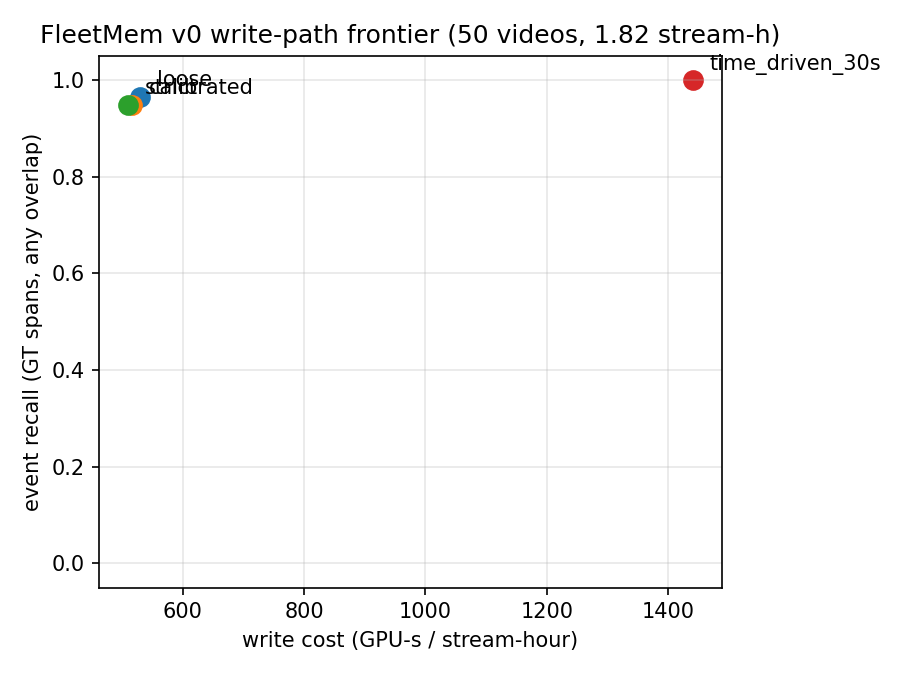
\includegraphics[width=0.9\textwidth]{figures/write_frontier.png}
\caption{Event-recall vs.\ write cost and storage on a 50-video stratified subset (59 ground-truth events). Event-driven gates reach recall 0.949--0.966 at 509--530 GPU-s/stream-hour (stride-1 tier-1 charge; stride 4 subtracts 264 GPU-s/stream-hour, Section~\ref{sec:exp-write}) and $\sim$1.2\,MB/stream-day; time-driven 30-s captioning (the Avas-style policy) reaches 1.000 at 1{,}442 GPU-s/stream-hour and 7.7\,MB/stream-day. Gate separation is small because tier-1 scores are bimodal on this subset (Section~\ref{sec:exp-write}).}
\label{fig:write-frontier}
\end{figure*}

\sys comprises a per-stream \emph{write ladder}, a \emph{tiered memory}, a \emph{fleet arbiter}, and a \emph{query path} (Figure~\ref{fig:write-frontier} previews the write economics). Every design choice below is justified by a measurement; cross-references point to the evidence.

\subsection{The write ladder: event-driven memory writes}
\label{sec:design-write}

Each stream is processed by a three-tier ladder; each tier gates the next, so expensive computation runs only where cheaper computation says it matters.

\paragraph{Tier 0: decode.} Frames are decoded on CPU (measured: 25{,}482 frames/s across 16 cores; 0.6\% of the GPU budget; Appendix~\ref{app:e0}). Decode is never the bottleneck at our scale and is excluded from GPU accounting.

\paragraph{Tier 1: salience.} A weakly-supervised anomaly scorer (VadCLIP~\cite{vadclip}, reproduced to within 0.0001 of its published AUC in our prior study) produces a per-clip score stream. Two measurements justify using it as a gate: tier-1 is 4--8$\times$ oversampled for detection (stride 4 costs $-$0.0014 AUC at 4$\times$ less compute), and its scores are strongly bimodal, so a calibrated gate is stable (Appendix~\ref{app:e0}). Events are formed as contiguous runs above gate $\tau=0.5$ with margin hysteresis $m=0.15$. \sys's production setting is stride 4: 89.8 GPU-s/stream-hour (the stride-1 setting, 354 GPU-s/stream-hour, buys back only 0.0014 AUC).

\paragraph{Tier 2: narration.} Gated events are narrated by Qwen2.5-VL-7B~\cite{qwen25vl} under a strict JSON schema (actors, actions, objects, location cues, one-sentence summary) plus a closed-taxonomy \emph{category tag} used as a retrieval feature. Three measured findings shape this tier (Section~\ref{sec:exp-grounded}): (i) neutral schema prompts avoid the alarmism we measured for judgment-style prompts; (ii) narrations are grounded (95.5\% of actions verified against frames by cross-model judging, 0.5\% hallucination); (iii) category labels must not be derived from narration text (40--62\% consistency) --- hence tags are a \emph{feature}, not a label, and the taxonomy is closed. Cost: 8.1\,s per event (schema, 8 frames), 154 GPU-s/stream-hour at measured event rates.

The ladder's write cost is \textbf{244 GPU-s/stream-hour} and 1.13\,MB/stream-day end-to-end with tier-1 at stride 4 (Section~\ref{sec:exp-write}; the stride-1 configuration we initially measured costs 508 GPU-s/stream-hour) --- versus 1{,}442 GPU-s/stream-hour and 7.7\,MB/stream-day for time-driven 30-s captioning at equal query machinery, and gigabytes per stream-day for KV retention.

\subsection{Tiered memory with tombstones}
\label{sec:design-memory}

Each event produces a layered record:
\begin{itemize}
\item \textbf{L0 --- metadata} (bytes): stream id, span, tier-1 score trajectory, gate levels passed, category tag.
\item \textbf{L1 --- narration + text embedding} (KBs): the schema record and a bge-small embedding of its text for retrieval. Appearance embeddings are deliberately excluded from the retrieval key: our in-system comparison shows appearance indexes lack event semantics (Section~\ref{sec:exp-tasti}), consistent with our earlier cross-camera analysis (Appendix~\ref{app:e0}).
\item \textbf{L2 --- optional segment embedding}: a second retrieval view (not used in this paper's main configuration).
\item \textbf{L3 --- raw-footage pointer}: the video itself is the cheapest memory tier (24/7 recording is standard practice); verification reads it at query time.
\end{itemize}

\paragraph{Eviction as compression.} When the storage budget $B_S$ binds, the eviction policy scores each record by salience, within-stream tag rarity, and marginal semantic coverage (a greedy facility-location-style selection that keeps a record only if it adds coverage relative to already-kept records). Evicted records are replaced by \emph{tombstones} --- compact stubs (time range, category histogram, count) --- that preserve aggregate answerability at near-zero bytes. Section~\ref{sec:exp-eviction} shows tombstones lift retrieval AP 3.5$\times$ against the strongest selection policy at 2\% retention (and equalize all policies --- the stubs carry the aggregate signal).

\subsection{The fleet arbiter: admission control, not ordering}
\label{sec:design-arbiter}

All streams' narration jobs enter one shared queue across the server's GPUs. Our measurements (Section~\ref{sec:exp-fleet}) show that under saturation, priority \emph{ordering} alone is indistinguishable from FCFS --- work-conserving queues process the same jobs regardless of order. The effective lever is \emph{admission control}: when the backlog exceeds a calibrated threshold, the arbiter \emph{sheds} incoming writes whose rank-normalized salience falls below the fleet's current percentile, while high-salience writes are always admitted. Optional fidelity degradation (4 frames instead of 8 per narration) further cuts the freshness tail ($\sim$1.6$\times$). The arbiter is deliberately a \emph{slow, fleet-level} controller: our prior study found per-window causal adaptation captures 0\% of oracle headroom (Appendix~\ref{app:e0}), so adaptation lives at the granularity where it works.

\subsection{The query path: retrieve, verify asymmetrically, or abstain}
\label{sec:design-query}

A natural-language query is embedded and matched against L1 embeddings and narration text (two channels, max-pooled). Per type: \emph{existence}/\emph{negation} --- threshold decision with a calibrated $\tau$ (calibrated once on a frozen 20\% split, then fixed); \emph{temporal} --- matched events return \emph{refined sub-spans} (inner-threshold runs plus peak-centered windows; Section~\ref{sec:exp-v01}); \emph{retrieval} --- ranked event list, with category tags as the dominant feature; \emph{cross-camera} --- set/count aggregation over per-camera results.

Verification against raw footage (L3) is available at $\sim$2 GPU-s/query, but our measurements show it is \emph{asymmetric}: it cuts negation false alarms 4.4--5.5$\times$ yet false-rejects real events when narrations are generic, so it is deployed as a precision operating point (negation FAR 0.08), not as a blanket confirmer (Section~\ref{sec:exp-v01}). The system can \emph{abstain} when retrieval confidence is low --- an outcome no surveyed baseline can express.

\subsection{Cost accounting as a first-class output}
\label{sec:design-cost}

Every run records GPU-seconds per pipeline stage, wall time, peak VRAM, and storage, pinned with configuration, environment, and code state (Appendix~\ref{app:repro}). \sys's outputs are \emph{frontiers}, not operating points: accuracy against GPU-s/stream-hour, bytes/stream-day, and GPU-s/query.
